\documentclass[11pt]{report}
\usepackage{graphicx}
\usepackage{amsmath}
\title{CS440 Project 2 Report}
\author{Douglas Gromek, Michael Comatas, Xiaoyu Sun}

\begin{document}
\maketitle

\section*{Naive Bayes}

Naive Bayes Rule: $$P(C|D) = \frac{P(D|C)P(C)}{P(D)}$$
$$P(D) = \sum _c P(D,C)$$
We know that $P(D)$ is a constant for all classes, so we could consider the equation above as:
$$P(C|D) \propto P(D|C)P(C)$$

where C stands for Class, D stands for Data. Thus, we only need to compute $P(D|C)$ and $P(C)$ in the implementation.

\subsection*{Digit - Implementation}

\paragraph{Training}
We first initialize 10 of 2D arrays with 0. Each array references as our models for 10 digits.
We know each image consists of symbols, by reading the training images, we save the image in the 2D array we have already. 
For example: \\

\begin{table}[h!]
\centering
\begin{tabular}{|c |c |c |c|} 
 \hline
0&0&0&0\\ 
 \hline
0&0&0&0\\ 
 \hline
0&0&0&0\\ 
 \hline
0&0&0&0\\ 
 \hline
\end{tabular}
\caption{Initial model for a digit}
\end{table}

Say we have two train images labeled 1, and the two images are saved below, as we mentioned, we would read the image, and if there is a symbol in a cell, we would save it  as a number.\\ 
\begin{table}[h!]
\centering
\begin{tabular}{|c |c |c |c|} 
 \hline
0&1&1&0\\ 
 \hline
0&1&1&0\\ 
 \hline
0&1&1&0\\ 
 \hline
0&1&1&0\\ 
 \hline
\end{tabular}
\caption{training image 1 with label 1}
\end{table}

\begin{table}[h!]
\centering
\begin{tabular}{|c |c |c |c|} 
 \hline
0&1&1&0\\ 
 \hline
0&1&1&0\\ 
 \hline
0&1&1&0\\ 
 \hline
0&1&1&0\\ 
 \hline
\end{tabular}
\caption{training image 2 with label 1}
\end{table}

After feed the model for digit 1 with the 2 training images above, the model for digit 1 would looks like this:
\begin{table}[h!]
\centering
\begin{tabular}{|c |c |c |c|} 
 \hline
0&2&2&0\\ 
 \hline
0&2&2&0\\ 
 \hline
0&2&2&0\\ 
 \hline
0&2&2&0\\ 
 \hline
\end{tabular}
\caption{training image with label 1}
\end{table}

After more and more images are feed to the model, we will have the model looks like this:
\begin{figure}[h]
\begin{center}
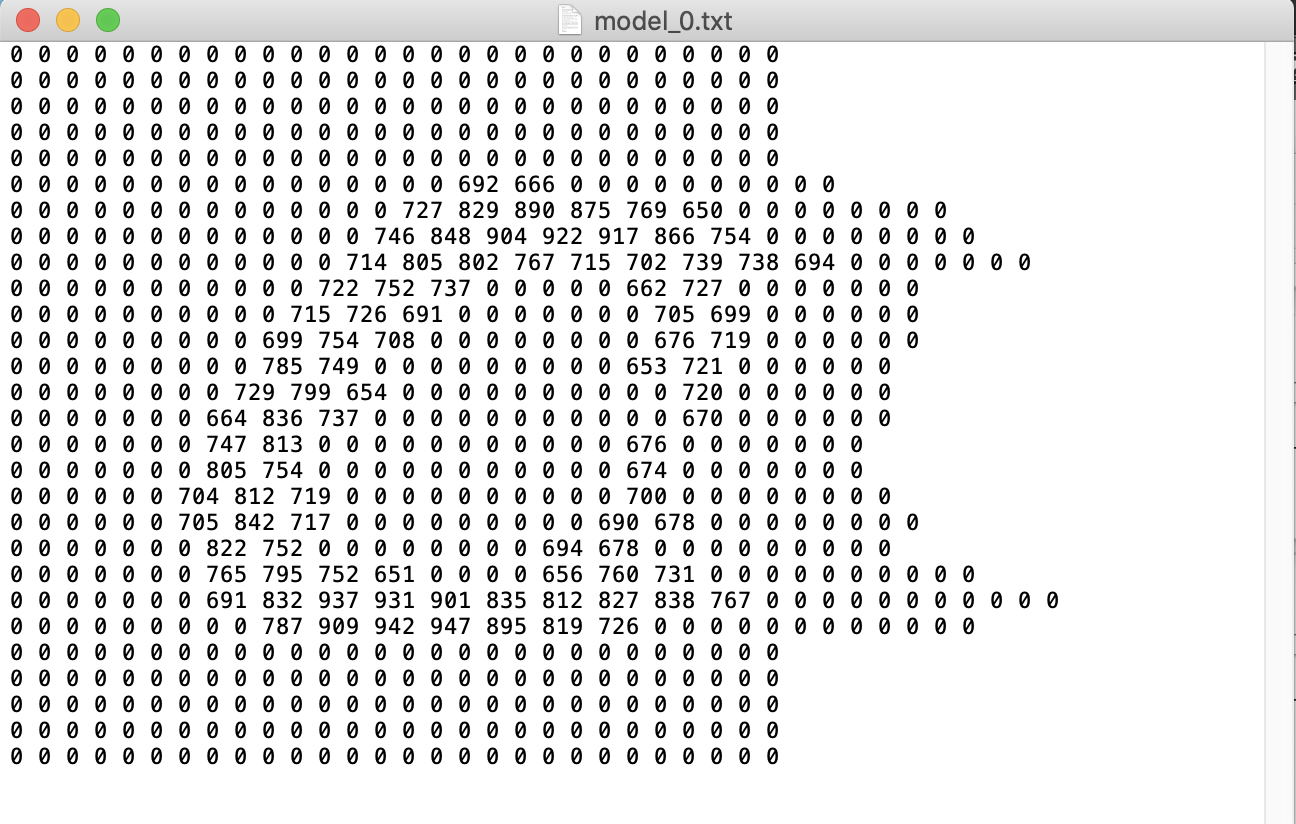
\includegraphics[width = 0.8\textwidth]{Bayes_digit_1.png} 
\end{center}
\caption{model for digit 1 after 100\% training data}
\end{figure}

We also filter out all the numbers that smaller than 650, such that the numbers left represent the densest area that digit 1 has appeared. 
\newpage

\paragraph{Prediction}
In order to make a prediction on one image, we test the image with all 10 models, then we pick the largest $P(D|C)$ among all the possibilities as the prediction. \\

\textbf{Steps:} \\

In order to compute $P(C)$:

$$P(C = x) = \frac{how\ many\ digit\ x\ in\ the\ data\ pool}{the\ total\ amount\ of\ digits}$$

such that we can get the frequency of the digit x. \\


Then we need to calculate $P(D|C)$: \\
$$P(D|C) = \Pi_{i=1}^m P(f_i|C)$$
For example: for $P(D|C=1)$, we loop through both the model for 1 and the test image, compare the common area between them,
$$P(f_n|C = 1) = \frac{common\ cells\ in\ row\ n}{total\ cells\ in\ row\ n}$$

\subsection*{Digit - Statistic}

\begin{figure}[h]
\begin{center}
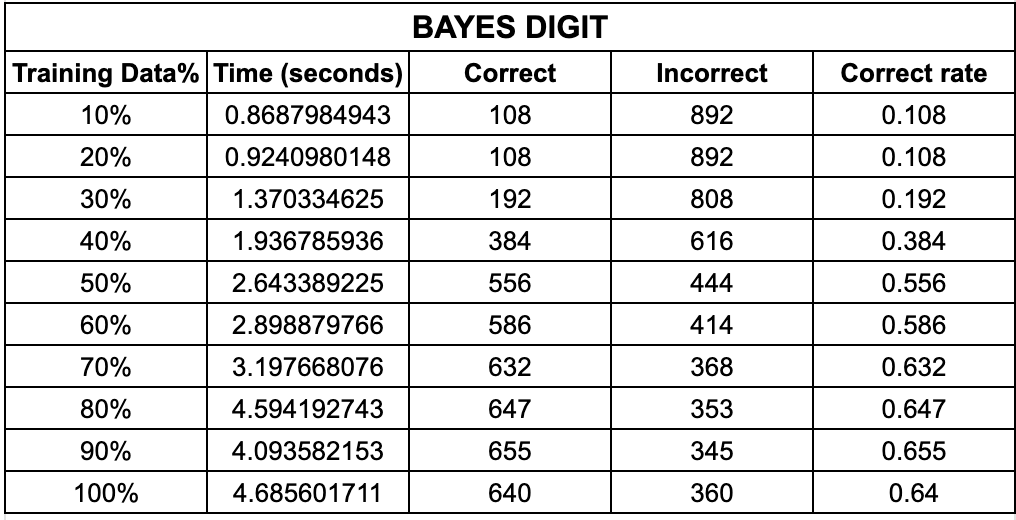
\includegraphics[scale=0.5]{Bayes_digit_statistic.png} 
\end{center}
\caption{Testing Data Collection for Digit}
\end{figure}
\newpage


\begin{figure}[]
\begin{center}
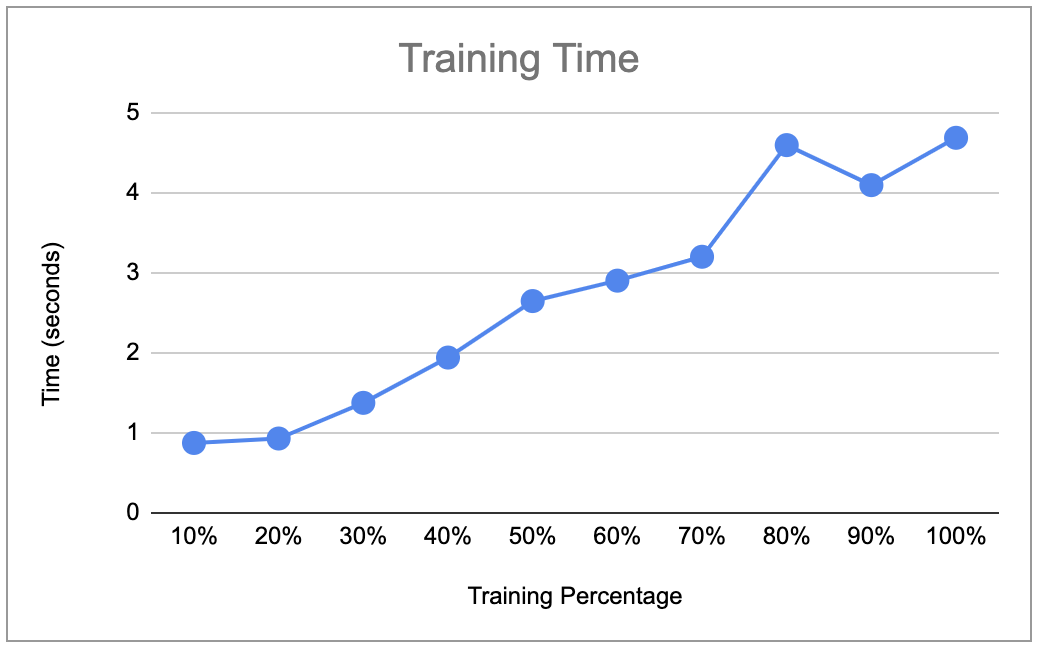
\includegraphics[scale=0.45]{Bayes_digit_traintime.png} 
\end{center}
\caption{Training Time vs. Training Data Percentage}
\end{figure}
From figure 3 we can tell that the more data we use, the longer the time it takes.\\

\begin{figure}[h]
\begin{center}
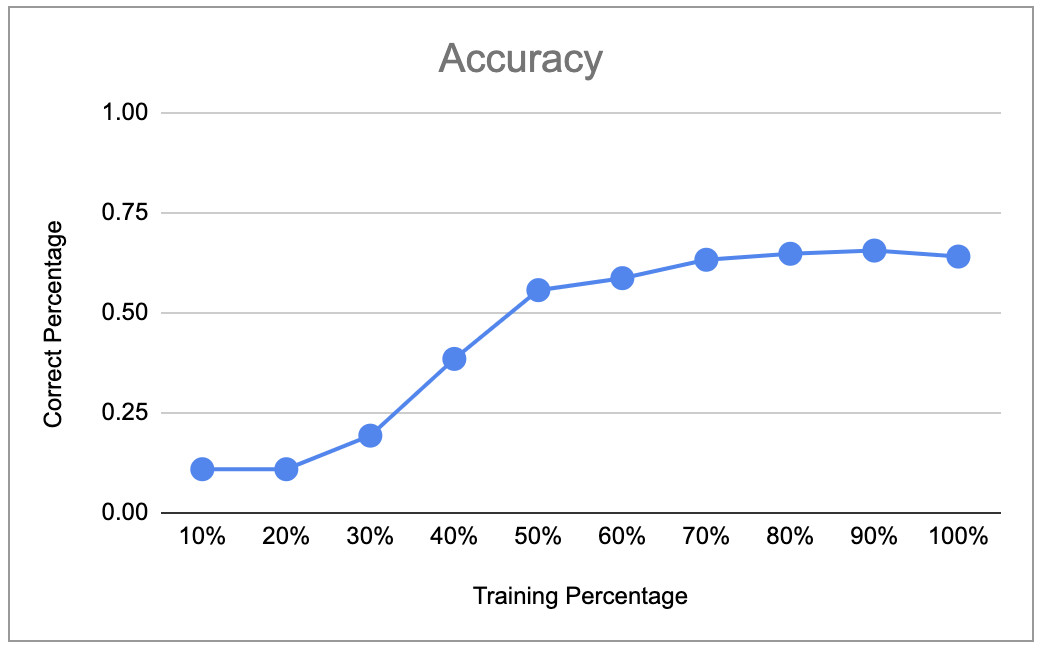
\includegraphics[scale=0.45]{Bayes_digit_accuracy.png} 
\end{center}
\caption{Correct percentage vs. Training Data Percentage}
\end{figure}


From figure 4 we can tell that the more training data we use, the prediction we made becomes more accurate. However, when the amount of data up to a certain number, the growth pace of the accuracy slows down. It might because of the limitation of our algorithm design, the maximum of the accuracy the feature can make is around 65\%, such that the accuracy stops changing significantly. 

\begin{figure}[h]
\begin{center}
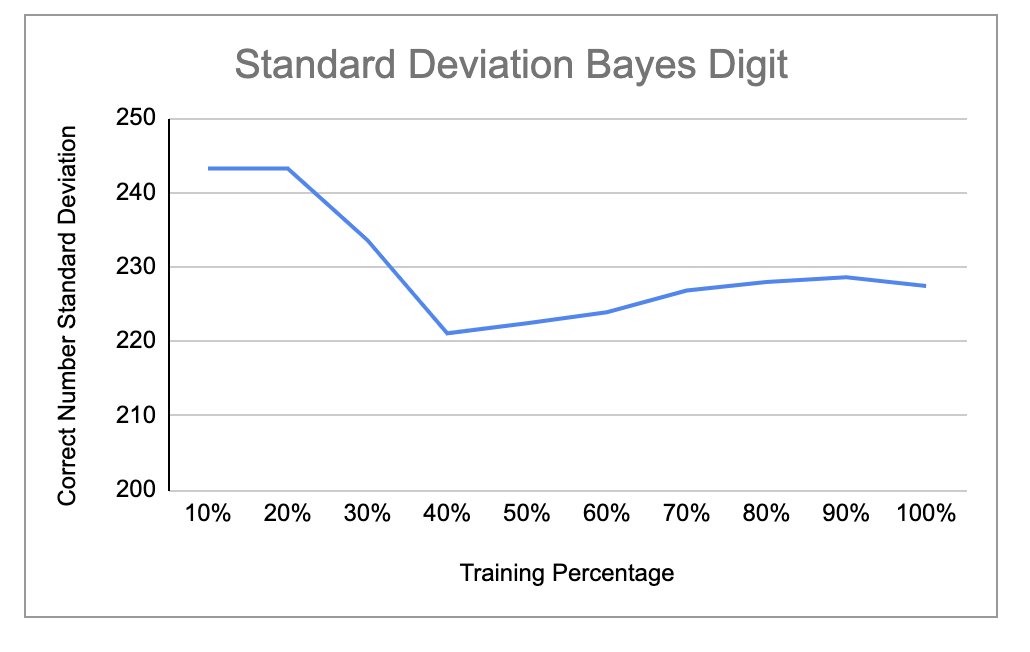
\includegraphics[scale=0.5]{Bayes_digit_SD.png} 
\end{center}
\caption{Standard Deviation for Bayes digit}
\end{figure}


From figure 5 we noticed the standard deviation tends to be inverse proportional to the amount of training data provided. After a certain amount of training data provided the standard deviation began to converge, for example around 40\% or 50\%. With less training data provided the standard deviation tended to be larger because there is a larger difference in accuracy. Then as the accuracy begins to be more precise the standard deviation converges. When the standard deviation would spike it was most likely because of overfitting, basically when the model "memorized" the figure rather than learning and "generalizing" to it.

\subsection*{Face - Implementation}

\paragraph{Training}
First we initialize 4 lists:

\begin{itemize}
\item 1. Hold the max row length for every non-face image
\item 2. Hold the max row length for every face image
\item 3. Hold the max column length for every non-face image
\item 4. Hold the max column length for every face image
\end{itemize}

We loop through all the training images, then populate above four lists. Then save it locally as a .txt file.

\paragraph{Prediction}
In order to make a prediction on one image, we get the max row and max column length 
values for  that image. We then we pick the largest $P(D|C)$ as the prediction. \\

\textbf{Steps:} 
Take face image as an example\\

In order to compute $P(C)$:

$$P(C_{face}) = \frac{total\ amount\ of\ faces}{the\ total\ amount\ of\ images}$$

such that we can get the frequency of faces appear. \\

Then we need to calculate $P(D|C)$: \\
$$P(D|C) = \Pi_{i=1}^m P(f_i|C)$$
In this case, $P(D|C_{face}) = P(f_{row}|C_{face})  \times P(f_{column}|C_{face}) $. \\

\noindent row:the times the max row length of current test image appears in the list2 above.\\
column:the times the max column length of current test image appears in the list4 above.
$$P(f_{row}|C_{face}) = \frac{row}{the\ length\ of\ list\ 2\ above}$$
$$P(f_{column}|C_{face}) = \frac{column}{the\ length\ of\ list\ 4\ above}$$

\newpage

\subsection*{Face - Statistic}

\begin{figure}[h]
\begin{center}
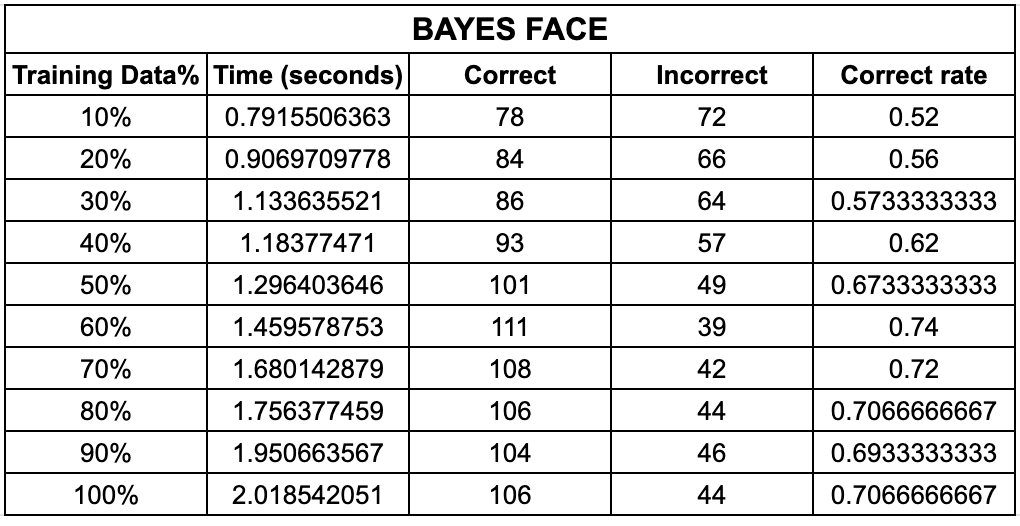
\includegraphics[scale=0.5]{Bayes_face_statistic.png} 
\end{center}
\caption{Testing Data Collection for Face}
\end{figure}

\begin{figure}[h]
\begin{center}
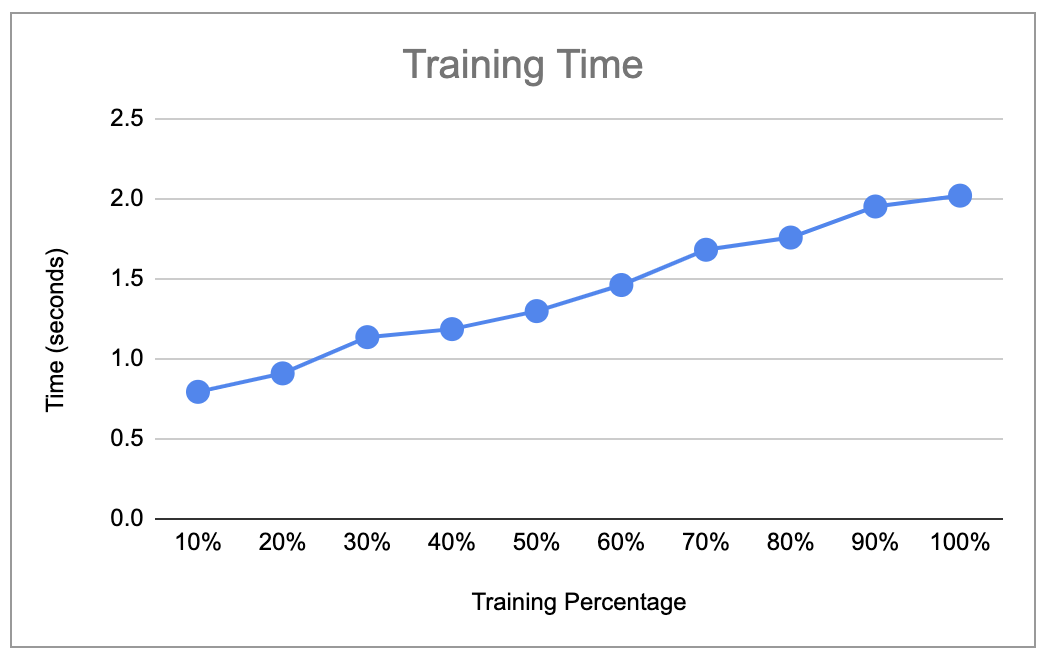
\includegraphics[scale=0.5]{Bayes_face_traintime.png} 
\end{center}
\caption{Training Time vs. Training Data Percentage}
\end{figure}
\newpage
\begin{figure}[t]
\begin{center}
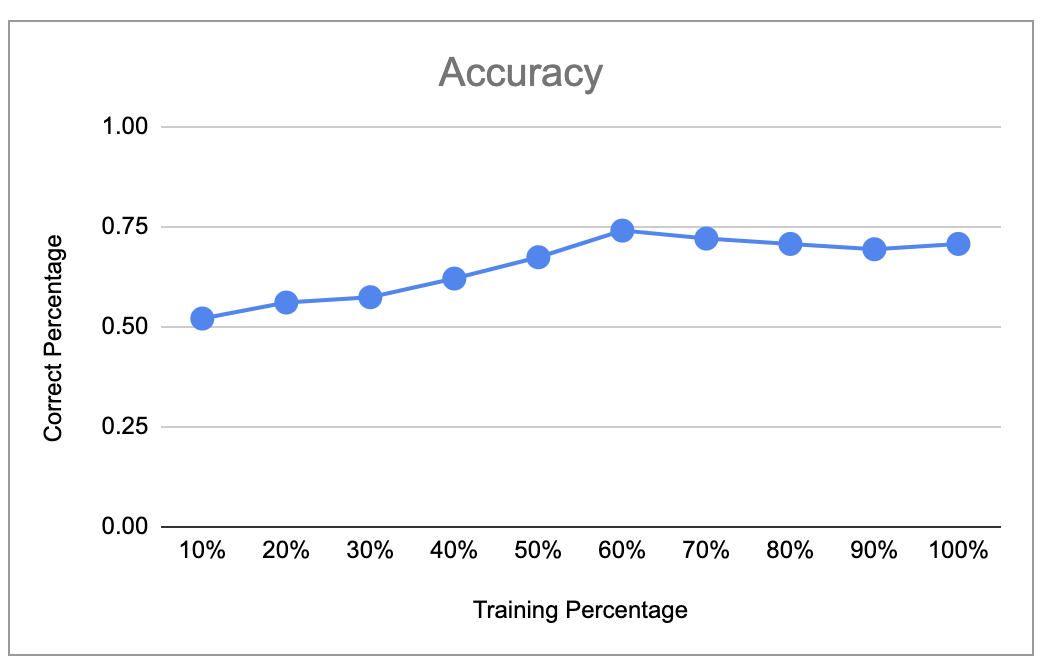
\includegraphics[scale=0.45]{Bayes_face_accuracy.png} 
\end{center}
\caption{Correct percentage vs. Training Data Percentage}
\end{figure}


From figure 7 we can tell that the more data we use, the longer the time it takes.\\

From figure 8 we can tell that the more training data we use, the prediction we made becomes more accurate. However, when the amount of data up to a certain number, the growth pace of the accuracy slows down. Same as the reason for digit classification, it might because of the limitation of our algorithm design, the maximum of the accuracy the feature can make is around 70\%, such that the accuracy stops changing significantly. 


\begin{figure}[h]
\begin{center}
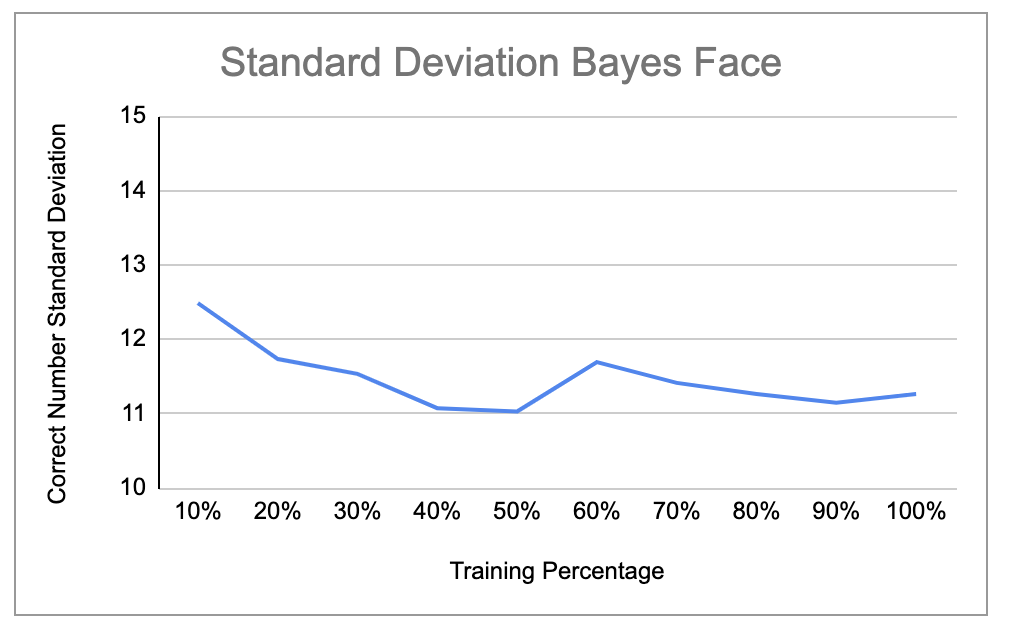
\includegraphics[scale=0.45]{Bayes_face_SD.png} 
\end{center}
\caption{Standard Deviation for Bayes face}
\end{figure}
\newpage


\section*{Perceptron}
\subsection*{Digit - Implementation}

\textbf{Training:} \\

1. We initialize the weight model by using random function to assign weights from -1 to 1. \\

2. For every training images, we loop through every row and every column of it, to get the following data:
 \begin{itemize}
\item How many "+" appears in row x
\item How many "\#" appears in row x
\item How many "+" appears in column y
\item How many "\#" appears in column y
\end{itemize}

We have a list of features that contains above data. Each of them is a feature, if the image's size is $x \times y$, such that as total, we have $2 \times x + 2 \times y $ features.\\


3. We use the equation below to calculate f value:
$$f(x_i, w) = w_0 + w_1\phi(x_i)+ w_2\phi(x_i) + ... + + w_l\phi(x_i)$$

For example, in this case, $\phi(x_i)$ with $w_2$ would be feature 2 we have, which is how many "\#" appears in row 0. \\


4. In order to adjust the weight model, we first calculate the f-value for all the 10 digits weight model, then pick the largest one as our prediction. In perceptron, the process of training is also a process of predicting. Then we compare the predict result to the actual label:
 \begin{itemize}
\item If the prediction is right and the f-value $<$ 0, then we adjust the all the weights of the prediction digit by:
$$w_0 = w_0 + 1$$
$$w_j = w_j + \phi(x_i)$$
\item If the prediction is wrong and the f-value $\geq 0$, then we adjust the all the weights of the prediction digit by:
$$w_0 = w_0 - 1$$
$$w_j = w_j - \phi(x_i)$$
Also adjust the all the weights of the actual label by:
$$w_0 = w_0 + 1$$
$$w_j = w_j + \phi(x_i)$$
\end{itemize}


\noindent \textbf{Prediction:} \\

This part has the same process as the training, the only diffrences: 
\begin{itemize}
\item 1.  We read the weigh model file that we save locally as the model. 
\item 2. After we get the prediction, we don't adjust the weight model.
\end{itemize}

We loop through the weights model for the 10 digits, and calculate the f-value by the following equation:
$$f(x_i, w) = w_0 + w_1\phi(x_i)+ w_2\phi(x_i) + ... + + w_l\phi(x_i)$$
Then we pick the largest one among the 10 f-values as our prediction.

\newpage
\subsection*{Digit - Statistic}

\begin{figure}[h]
\begin{center}
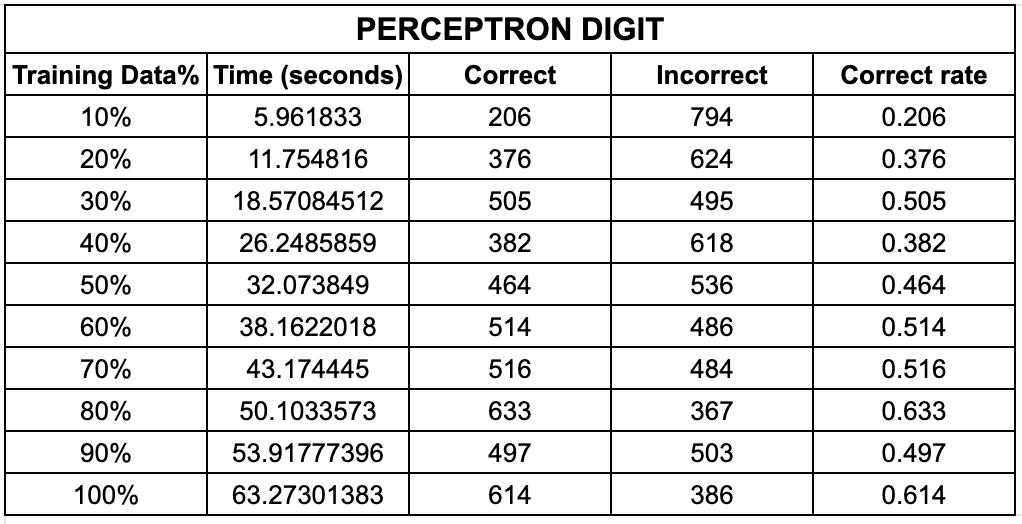
\includegraphics[scale=0.5]{Perceptron_digit_statistic.png} 
\end{center}
\caption{Testing Data Collection for Digit}
\end{figure}

\begin{figure}[h]
\begin{center}
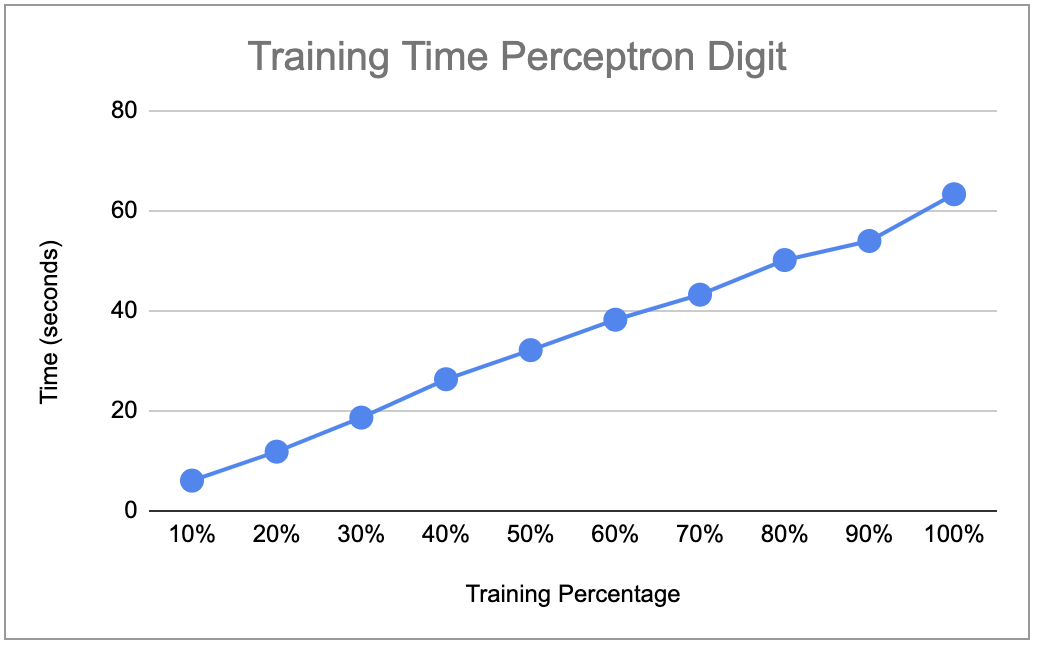
\includegraphics[scale=0.5]{Perceptron_digit_traintime.png} 
\end{center}
\caption{Training Time vs. Training Data Percentage}
\end{figure}
\newpage
\begin{figure}[t]
\begin{center}
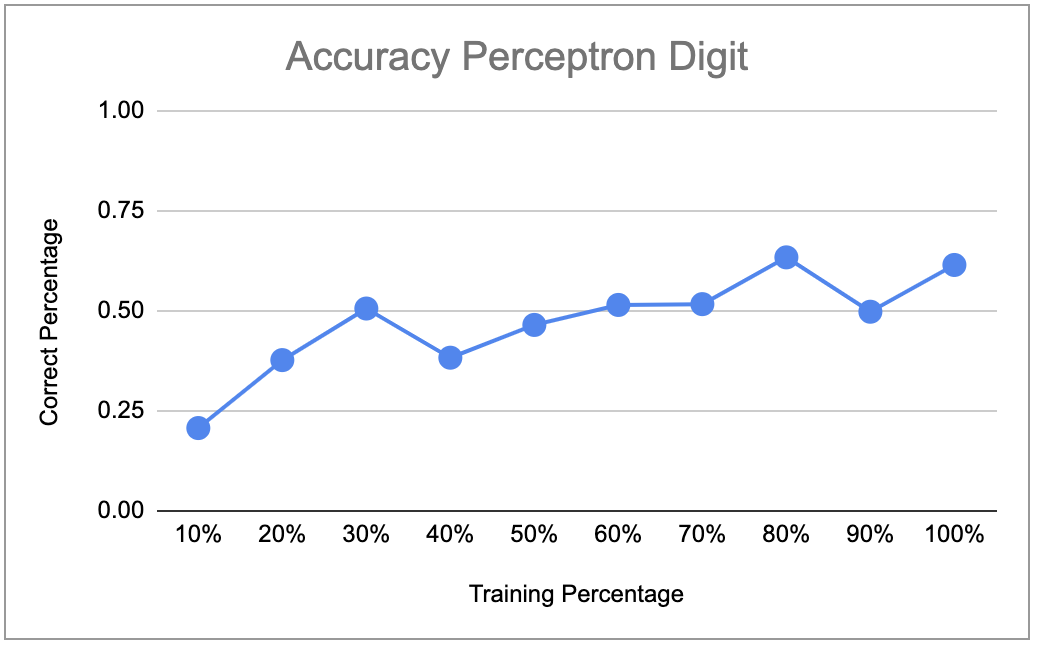
\includegraphics[scale=0.45]{Perceptron_digit_accuracy.png} 
\end{center}
\caption{Correct percentage vs. Training Data Percentage}
\end{figure}

From figure 11 we can tell that the more data we use, the longer the time it takes.\\

From figure 12 we can tell that the more training data we use, the prediction we made becomes more accurate. However, when the amount of data up to a certain number, the growth pace of the accuracy slows down. Same as the reason before, it might because of the limitation of our algorithm design, the maximum of the accuracy the feature can make is around 60\%, such that the accuracy stops changing significantly. 

\begin{figure}[h]
\begin{center}
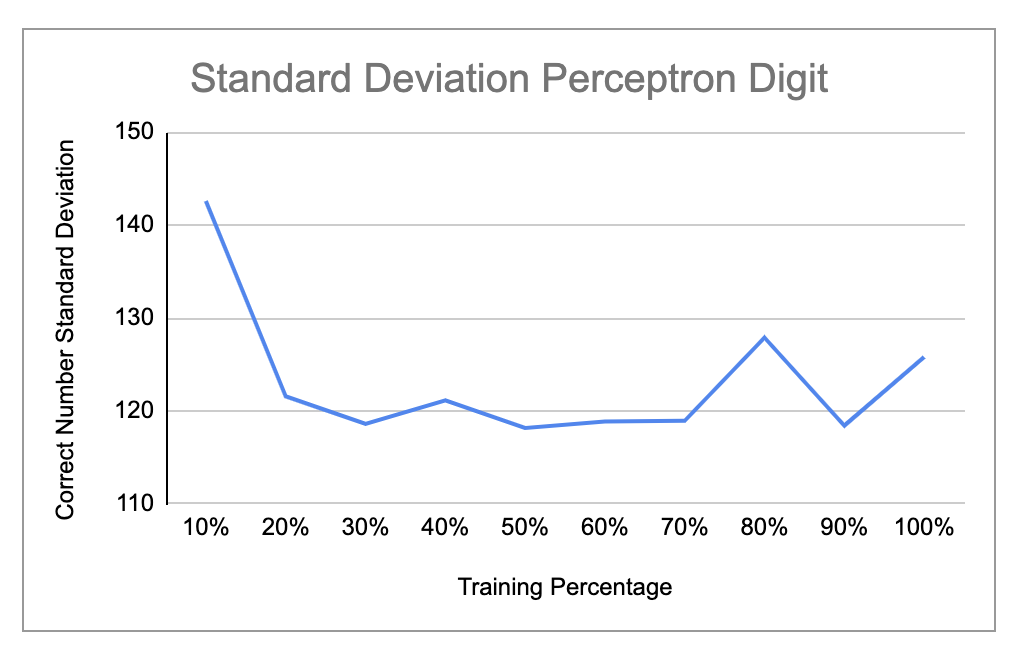
\includegraphics[scale=0.45]{Perceptron_digit_SD.png} 
\end{center}
\caption{Standard Deviation for Perceptron digit}
\end{figure}
\newpage

\subsection*{Face - Implementation}
\textbf{Training:} \\

1. We initialize the weight model by using random function to assign weights from -1 to 1. \\

2. We loop through all the train images, then get the max lengths for row x among all the images, then store them somewhere. Thus the number of features we have equals the number of rows this image has.

3. We use the equation below to calculate f value:
$$f(x_i, w) = w_0 + w_1\phi(x_i)+ w_2\phi(x_i) + ... + + w_l\phi(x_i)$$

For example, in this case, $\phi(x_i)$ with $w_2$ would be feature 2 we have, which is the max lengths for row 2 among all the images.. \\


4. In order to adjust the weight model, we first calculate the f-value for face and non-face weight models, then pick the larger one as our prediction. In perceptron, the process of training is also a process of predicting. Then we compare the predict result to the actual label:
 \begin{itemize}
\item If the prediction is right and the f-value $<$ 0, then we adjust the all the weights of the prediction digit by:
$$w_0 = w_0 + 1$$
$$w_j = w_j + \phi(x_i)$$
\item If the prediction is wrong and the f-value $\geq 0$, then we adjust the all the weights of the prediction digit by:
$$w_0 = w_0 - 1$$
$$w_j = w_j - \phi(x_i)$$
Also adjust the all the weights of the actual label by:
$$w_0 = w_0 + 1$$
$$w_j = w_j + \phi(x_i)$$
\end{itemize}


\noindent \textbf{Prediction:} \\

This part has the same process as the training, the only diffrences: 
\begin{itemize}
\item 1.  We read the weigh model file that we save locally as the model. 
\item 2. After we get the prediction, we don't adjust the weight model.
\end{itemize}

We loop through the weights model of face and non-face, and calculate the f-value by the following equation:
$$f(x_i, w) = w_0 + w_1\phi(x_i)+ w_2\phi(x_i) + ... + + w_l\phi(x_i)$$
Then we pick the larger one as our prediction.

\subsection*{Face - Statistic}

\begin{figure}[h]
\begin{center}
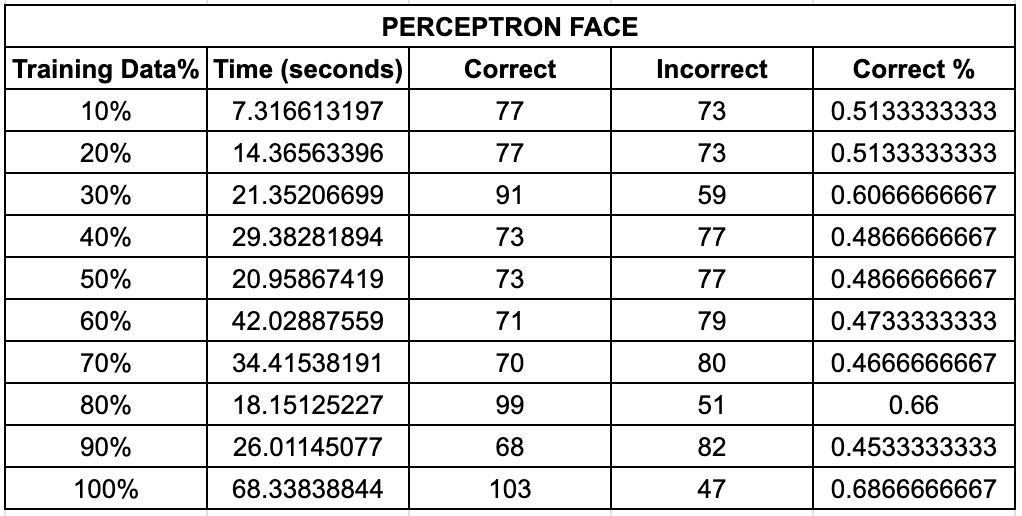
\includegraphics[scale=0.5]{Perceptron_face_statistic.png} 
\end{center}
\caption{Testing Data Collection for Face}
\end{figure}

\begin{figure}[h]
\begin{center}
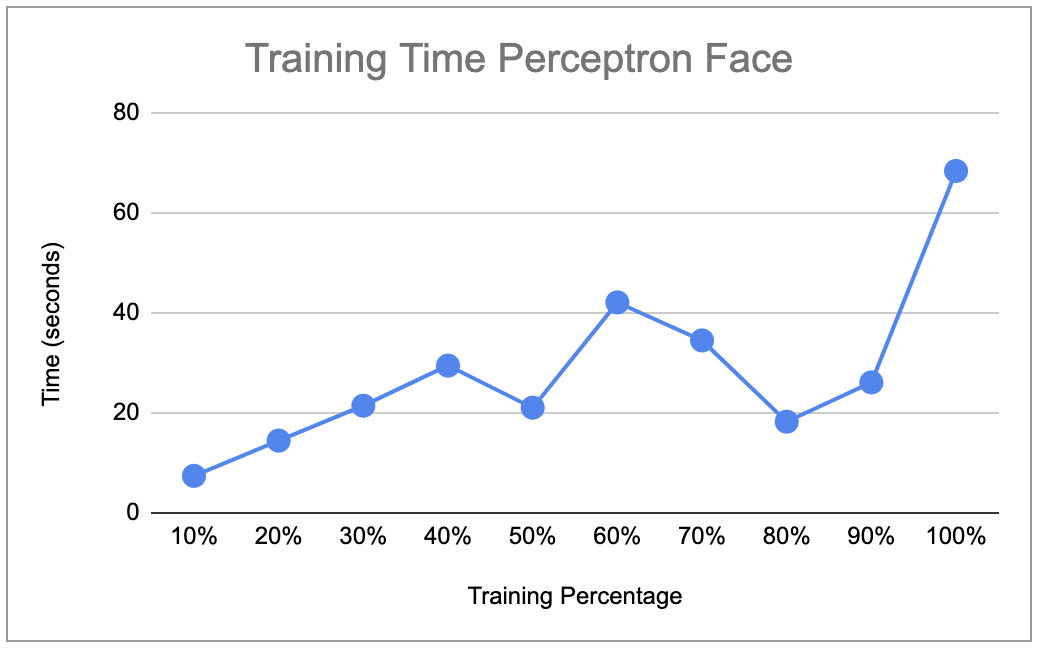
\includegraphics[scale=0.5]{Perceptron_face_traintime.png} 
\end{center}
\caption{Training Time vs. Training Data Percentage}
\end{figure}
\newpage
\begin{figure}[t]
\begin{center}
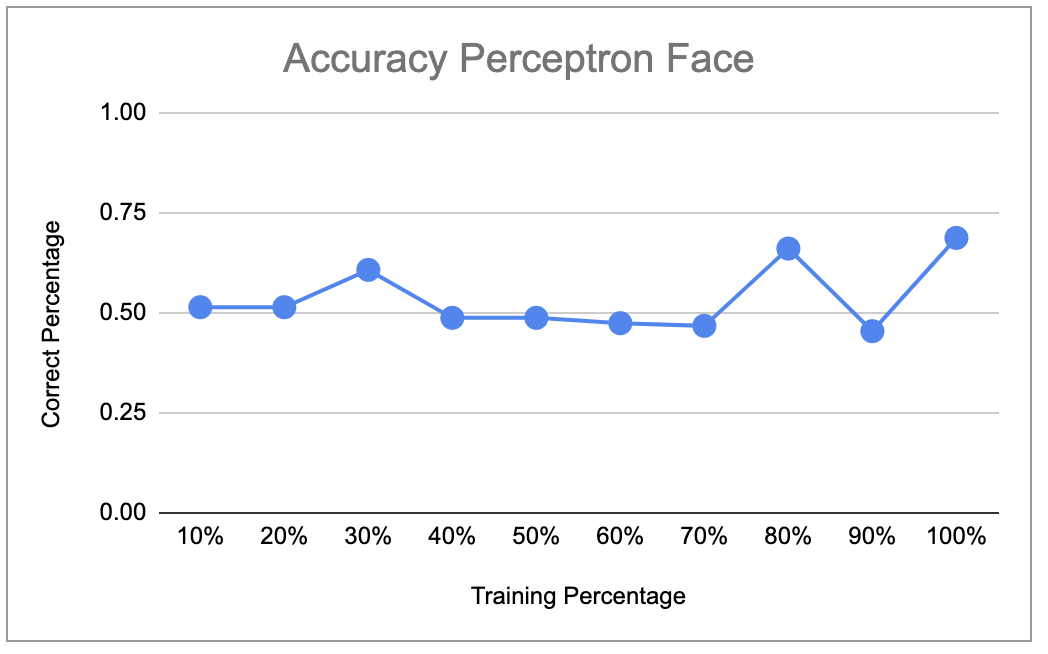
\includegraphics[scale=0.5]{Perceptron_face_accuracy.png} 
\end{center}
\caption{Correct percentage vs. Training Data Percentage}
\end{figure}

From figure 15 we can tell that the more data we use, the longer the time it takes.\\

From figure 16 we can tell that the more training data we use, the prediction we made becomes more accurate. However, from 40\% to 70\% the accuracy is lower than the two sides, the reason could that part of data is biased.

\begin{figure}[h]
\begin{center}
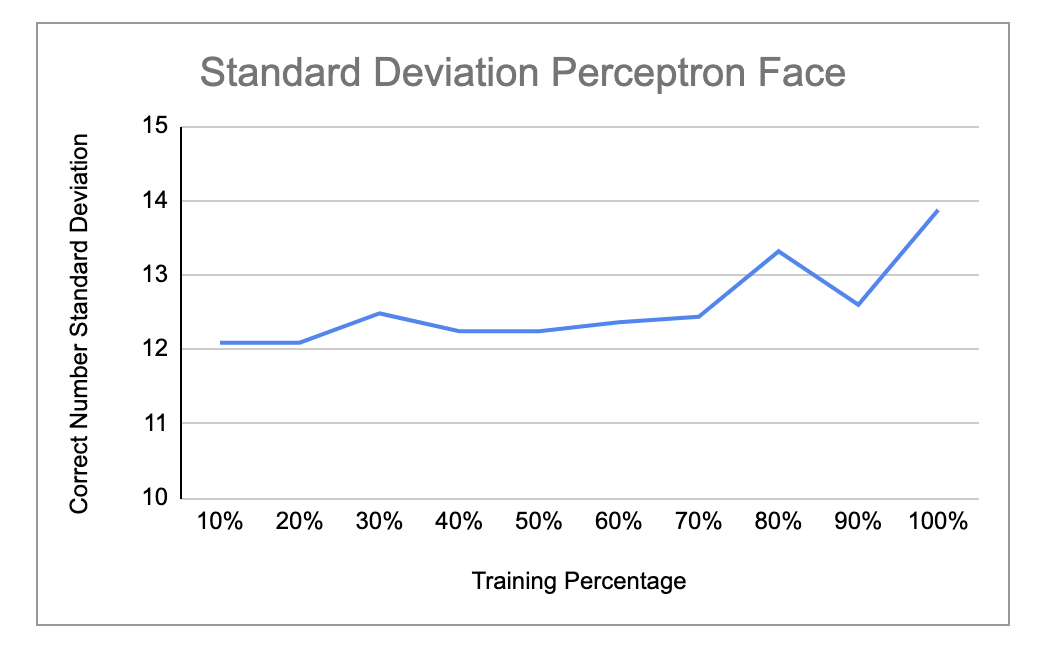
\includegraphics[scale=0.5]{Perceptron_face_SD.png} 
\end{center}
\caption{Standard Deviation for Perceptron face}
\end{figure}

\end{document}